\chapter{User documentation}
\label{ch:user}

The Wrangler Language Server is a tool that enables developers to use the refactorings defined in Wrangler through the Erlang Language Server.

In this document, the set up, the examples and the screenshots are presented for the Visual Studio Code text editor.

Installing Wrangler includes installing Wrangler LS, but it is started and run by Erlang LS (which is started and run by the development tool).
In order to use Wrangler LS, further configuration is needed in the Erlang LS.

\section{System requirements}

The system requirements for the Wrangler LS is constrained by the underlying tools' (namely the Erlang LS, Wrangler itself and the development tool: Visual Studio Code) requirements:

\begin{enumerate}
    \item Hardware requirements: \todo{Check hardware requirements}
    \begin{itemize}
        \item 1.6 GHz or faster processor is recommended by Visual Studio Code
        \cite{VSCodeRequirements}
        \item 1 GB of RAM is recommended by Visual Studio Code \cite{VSCodeRequirements}
        \item 500 MB free space on the hard drive is needed to install Visual Studio Code, Wrangler and the Erlang
    \end{itemize}
    \item Software requirements:
    \begin{itemize}
        \item GNU/Linux or MacOS operating system \footnote{The Microsoft Windows operating system is restricted only by Wrangler`s currently outdated Windows installer.}
        \item Erlang/OTP 24.0 or newer version.
        \item \todo{Wrangler requirements - gcc?}
    \end{itemize}
    \item Other requirements:
    \begin{itemize}
        \item Administrator privileges on the operating system.
    \end{itemize}
\end{enumerate}


\section{Installing and configuration}

Wrangler's codebase, Visual Studio Code's installer and a Visual Studio Code extension installer (.vsix file) for the Erlang LS can be found in the thesis's appendix.

Alternatively, all necessary files can be downloaded from the websites of each tool \cite{WranglerGitHub, VSCodeDownload, ELSExtension}

\subsection{Installing Wrangler}

Wrangler needs to be compiled and installed with the command below \ref{src:install}.

\lstset{caption={Build and install Wrangler}, label=src:install}
\begin{lstlisting}[language=bash]
  ./configure && make && sudo make install
\end{lstlisting}

More information and options about installing Wrangler can be found in the \emph{INSTALL} file located at Wrangler`s root directory.

As mentioned, installing Wrangler will also install the Wrangler Language Server.

\subsection{Installing Visual Studio Code}

Installing Visual Studio Code with its installer should be straightforward, but a detailed walk-through is available about installation process at their website \cite{VSCodeDownload}.

\subsection{Installing the Erlang Language Server}

Once Visual Studio Code is installed, Erlang LS can be installed with the command below \ref{src:install-els}, providing the path to the \tt .vsix\rm\ file.

\lstset{caption={install Wrangler}, label=src:install-els}
\begin{lstlisting}[language=bash]
  code --install-extension els.vsix
\end{lstlisting}

Alternatively, the extension can be up automatically downloaded and installed from Visual Studio Code's marketplace \cite{ELSInstall}.

\subsection{Configuring the Wrangler Language Server}

A configuration file named \emph{erlang\_ls.config} should be placed in the root directory of every project where Wrangler needs to be used.
\begin{note}
Global configuration options are also available, as discussed on Erlang LS's website \cite{ELSConfig}.
\end{note}

A configuration example \ref{src:wrangler-config-example} and the description of the parameters \ref{tab:wrangler-config-descr} are shown below.

\lstset{caption={erlang\_ls.config example}, label=src:wrangler-config-example}
\begin{lstlisting}
wrangler:
  enabled: true
  path: "/path/to/wrangler/ebin" 
  tab_with: 8
  enabled_refactorings:
    - "comment-out-spec"
    - "fold-expression"
    - "generalise-fun"
    - "move-fun"
    - "new-fun"
    - "new-macro"
    - "new-var"
    - "rename-fun2"
    - "rename-var"
\end{lstlisting}


\begin{table}[H]
	\centering
	\begin{tabular}{ | m{0.3\textwidth} | m{0.1\textwidth} | m{0.5\textwidth} | }
		\hline
		\textbf{Parameter} & \textbf{Type} & \textbf{Description} \\
		\hline \hline
		\emph{enabled} & \emph{boolean} & \emph{true} if Wrangler should be enabled or \emph{false} if not. \\
		\hline
		\emph{path} & \emph{string?} & Only necessary when Wrangler is not installed system-wide. A path to Wrangler's compiled \emph{ebin} folder should be set. \\
		\hline
		\emph{tab\_with} & \emph{integer?} & The used tabulator width in the project. Defaults to 8 if not provided. \\
		\hline
		\emph{enabled\_refactorings} & \emph{string[]} & All the Wrangler refactoring`s identification values that are enabled.\\
		\hline
	\end{tabular}
	\caption{Description of the configuration parameters}
	\label{tab:wrangler-config-descr}
\end{table}

Further configuration options for the Erlang Language Server can be found at their website \cite{ELSConfig}.

\section{Usage}

The Erlang Language Server starts automatically when an Erlang file is opened in the code editor. If Wrangler is enabled, the Erlang LS loads and starts it during initialization. After that, the refactorings should be accessible.

We classify the supported refactorings into two (plus one) groups based on their user input needs. We distinguish refactorings that require a simple value as its input (for example, a new argument's name) and refactorings for which simple inputs are not enough. In this paper, we call these groups \emph{simple} and \emph{complex} refactorings\footnote{The appelations do not imply any relation with the complexity of the refactorings' implementation.}. 

There is also a third category for special, module related refactorings described below.

In the sections below, after presenting the general use cases of the refactorings depending on the mentioned input types, the list of the supported refactorings are shown. In the list, after each refactoring's name, their identification value is presented, along with a brief description, their precondition, side effect(s) and an example. The preconditions show what the user need to do to get the refactoring offered by the language server.

\subsection{Simple refactorings}
\label{src:simple-ref}

The refactorings can be initiated when a certain code piece is highlighted or the cursor is set to a specific location. Then, the possible refactorings appear in the form of code actions from which the user can choose from \ref{fig:codeactions}.

\begin{figure}[H]
	\centering
	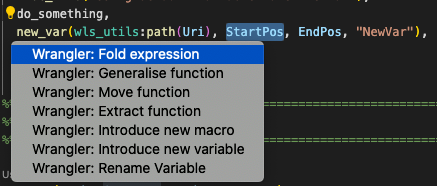
\includegraphics[width=1\textwidth]{images/code_actions.png}
	\caption{Code Actions showing the possible refactorings.}
	\label{fig:codeactions}
\end{figure}

These refactorings are based on text inputs. An input field that accepts valid erlang atoms or variables appear when the refactorings are selected \ref{fig:input}. On invalid input, a red error message appears \ref{fig:input-invalid}

\begin{figure}[H]
	\centering
	
\includegraphics[width=1\textwidth]{images/valid_input.png}
	\caption{Input field for Erlang atoms}
	\label{fig:input}
\end{figure}

\begin{figure}[H]
	\centering
	
\includegraphics[width=1\textwidth]{images/valid_input.png}
	\caption{Invalid input}
	\label{fig:input-invalid}
\end{figure}


In some cases, a file name has to be chosen with the a file selector menu based on the system.

\begin{figure}[H]
	\centering
	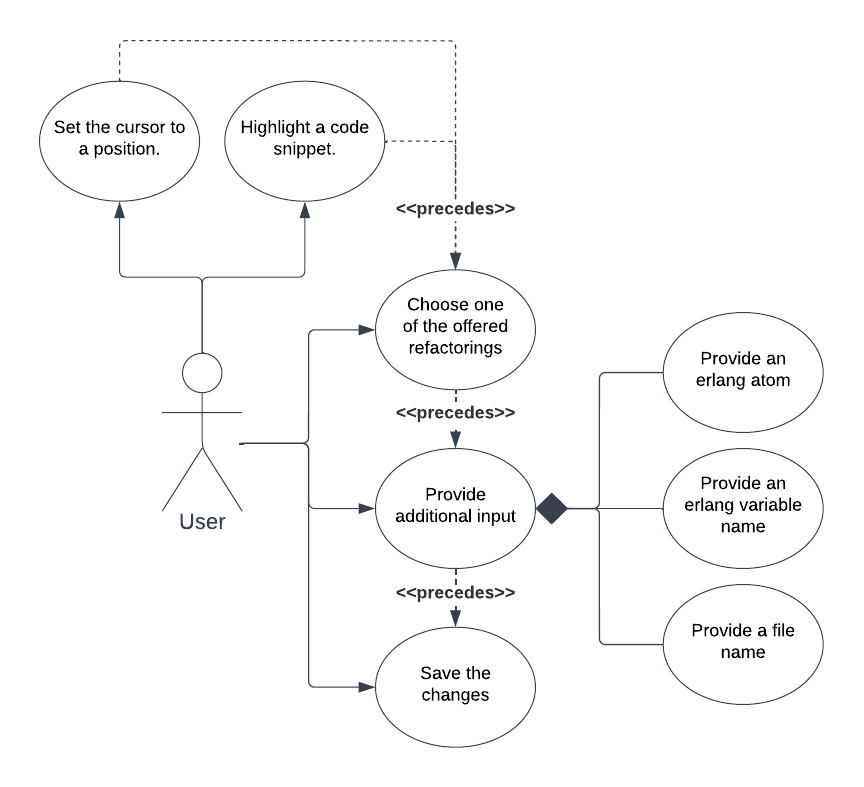
\includegraphics[width=1\textwidth]{images/use_case_1.png}
	\caption{Use case diagram for simple refactorings}
	\label{fig:usecase}
\end{figure}

\begin{description}
	\item[Generalise function / \textit{generalise-fun}:] 
	Refactor the highlighted expression as the function's new argument
	\\Precondition: highlight an expression.
	\\Asked user input: A variable name for the function's new argument. 
	\\Before refactoring:
	\begin{figure}[H]
	\centering
	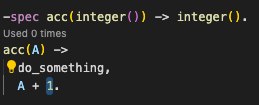
\includegraphics[]{images/gen_before.png}
    \end{figure}
	After refactoring:
	\begin{figure}[H]
	\centering
	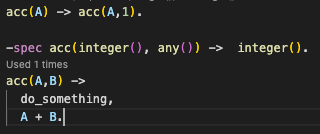
\includegraphics[]{images/gen_after.png}
    \end{figure}
	Side effect: The preserve the behaviour, the original function clause is modified.
	\item[Introduce new variable / \textit{new-var}] Introduce a new variable with the value of the highlighted expression.
	\\Precondition: highlight an expression.
	\\Asked user input: A variable name for the function's new argument. 
	\\Before refactoring:
	\begin{figure}[H]
	\centering
	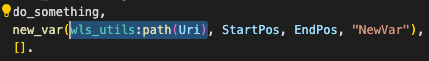
\includegraphics[]{images/new_var_before.png}
    \end{figure}
	After refactoring:
	\begin{figure}[H]
	\centering
	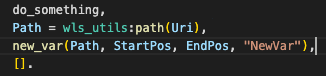
\includegraphics[]{images/new_var_after.png}
    \end{figure}
	Side effect: The original expression gets replaced by the new variable.
	\item[Move function / \textit{move-fun}] Move a function definition from its current module to another module.
	\\Precondition: set the cursor to a function name or inside its definition.
	\\Asked user input: The file where the function definition should be moved. 
	Side effect: It changes all function calls in the search paths to the new module.
	\item[Extract function / \textit{new-fun}] Introduce a new function definition to represent a selected expression sequence inside an existing function. 
	\\Precondition: highlight an expression sequence.
	\\Asked user input: A variable name for the new function's name. 
	\\Before refactoring:
	\begin{figure}[H]
	\centering
	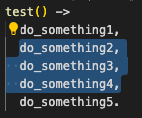
\includegraphics[]{images/extract_before.png}
    \end{figure}
	After refactoring:
	\begin{figure}[H]
	\centering
	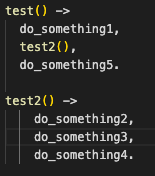
\includegraphics[]{images/extract_after.png}
    \end{figure}
	Side effect: The selected sequence of expressions is replaced by a call of the new function.
	\item[New macro / \textit{new-macro}] Define a macro to represent a selected sequence of expressions or patterns.
	\\Precondition: highlight an expression or pattern list.
	\\Asked user input: The new macro's name. 
	\begin{figure}[H]
	\centering
	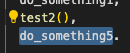
\includegraphics[]{images/macro_before.png}
    \end{figure}
	After refactoring:
	\begin{figure}[H]
	\centering
	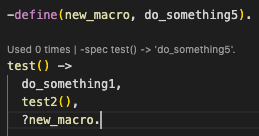
\includegraphics[]{images/macro_after.png}
    \end{figure}
	Side effect: The selected expressions or patterns are replaced by the new macro.
	\item[Rename function / \textit{rename-fun2}] Rename a function.
	\\Precondition: set the cursor position to a function name.
	\\Asked user input: A name for the function's new name. 
	\\Before refactoring:
	\begin{figure}[H]
	\centering
	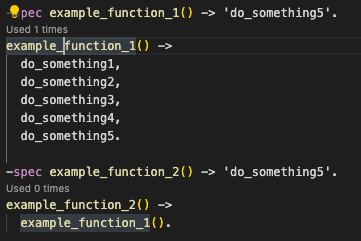
\includegraphics[]{images/rename_fun_before.png}
    \end{figure}
	After refactoring:
	\begin{figure}[H]
	\centering
	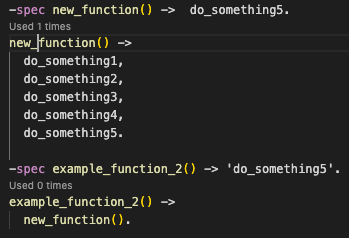
\includegraphics[]{images/rename_fun_after.png}
    \end{figure}
	Side effect: All the function calls and references are changed (including exports and specs).
	\item[Rename variable / \textit{rename-var}] Rename a variable.
	\\Precondition: highlight or set the cursor position to a variable.
	\\Asked user input: The variable's new name. 
    \begin{figure}[H]
	\centering
	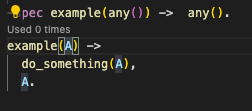
\includegraphics[]{images/rename_var_before.png}
    \end{figure}
	After refactoring:
	\begin{figure}[H]
	\centering
	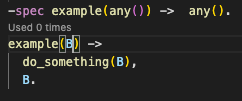
\includegraphics[]{images/rename_var_after.png}
    \end{figure}
	Side effect: The variable changes everywhere where it is used.
\end{description}

\subsubsection{Possible errors}

Various errors can be thrown in Wrangler during refactorings. These may occur because Wrangler is unable to determine whether it can safely perform the modifications, or because the preconditions for refactorings are not met.
If an error is triggered, the changes will be reverted to the code's original state and an error message describing the cause appears for the user \ref{fig:error}.

\begin{figure}[H]
\centering
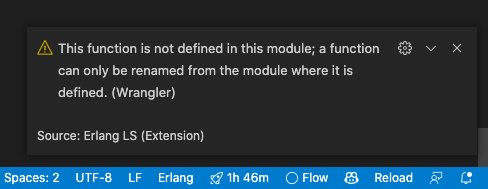
\includegraphics[width=1\textwidth]{images/errors.png}
\caption{An example error message for renaming functions.}
\label{fig:error}
\end{figure}

\subsection{Complex refactorings}

Complex refactorings differ from simple refactorings only in the way the input is requested. Everything else described in the previous section \ref{src:simple-ref} applies to them also.

Instead of requesting text input, the file to be modified transforms into a form we call Wrangler Forms.

The refactorings using these forms work by allowing the user to select each option where refactoring can be applied. These refactoring candidates get highlighted in the file and buttons (called code lenses) appear above each of them with which the refactorings can be executed or the form can be closed.

\begin{figure}[H]
	\centering
	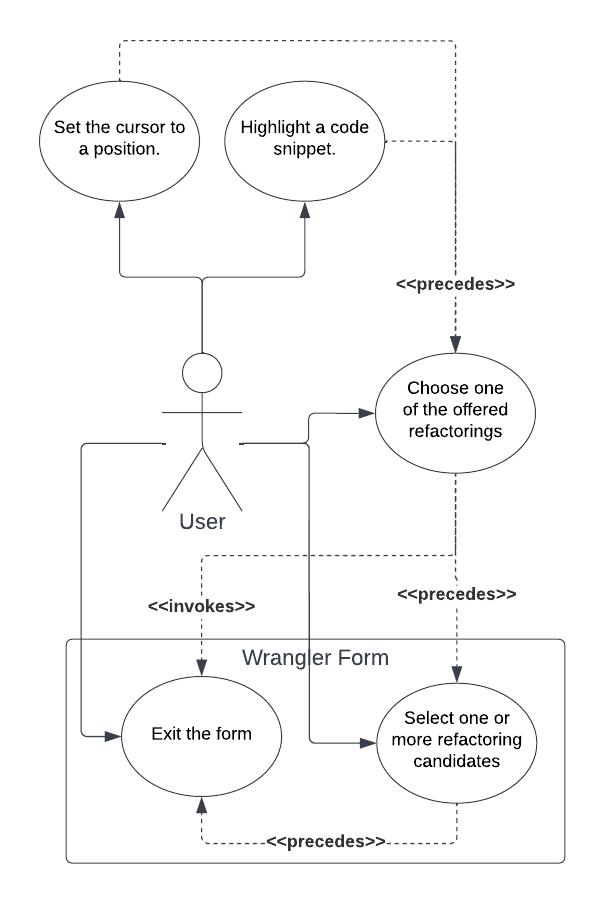
\includegraphics[width=1\textwidth]{images/use_case_2.png}
	\caption{Use case diagram for complex refactorings using Wrangler Forms}
	\label{fig:usecase2}
\end{figure}


Currently, expression folding uses these format. With fold, a function


\todo{Fold refactoring}

\subsection{Other refactorings}

\todo{comment out spec refactoring}